\section{Resumo}

\begin{frame}{Bellman Equation}
    Em Processos de Decisão de Markov:
    \begin{itemize}
        \item A \alert{equação de Bellman é uma recursão para recompensa esperada}.
        \begin{itemize}
            \item E.G. A recompensa esperada por estar em um estado particular s e seguir um política fica $\pi$ tem a equação de Bellman:
            $$V^{\pi}(s) = R(s, \pi(s)) + \gamma \sum_{s'}{P[s'|s,\pi(s)]V^{\pi}(s')}$$
        \end{itemize}
    \end{itemize}
    
    \begin{itemize}
        \item A equação para a política ótima refere-se à \alert{Equação Ótima de Bellman}.
        $$V^*(s) = \max_{a}{R(s,a) + \gamma \sum_{s'}{P(s'|s,a)V^*(s')}}$$
    \end{itemize}
\end{frame}

\begin{frame}{Softmax - Exploração}
    Bias action selection towards current estimate based on \alert{temperature} $\tau$. $\tau \rightarrow 0$ is greedy action selection.
    $$\pi(a) = \frac{e^{Q(a)/\tau}}{\sum_{a'}{e^{Q(a')/\tau}}}$$
\end{frame}

\begin{frame}{Framework de Aprendizado por Reforço (MDP)}
    \begin{figure}
        \centering
        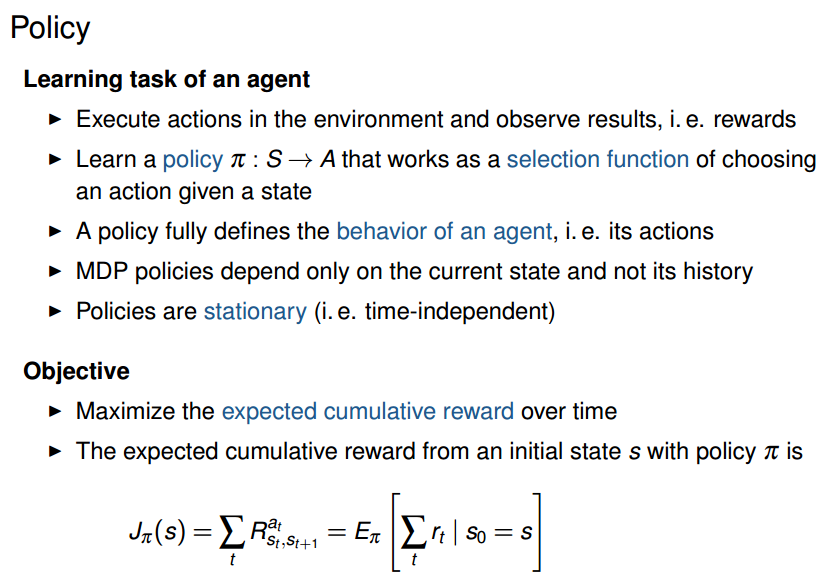
\includegraphics[width=0.7\textwidth]{img/policy.png}
        \caption{Caption}
        \label{fig:my_label}
    \end{figure}
\end{frame}

\begin{frame}{Framework de Aprendizado por Reforço (MDP)}
    \begin{figure}
        \centering
        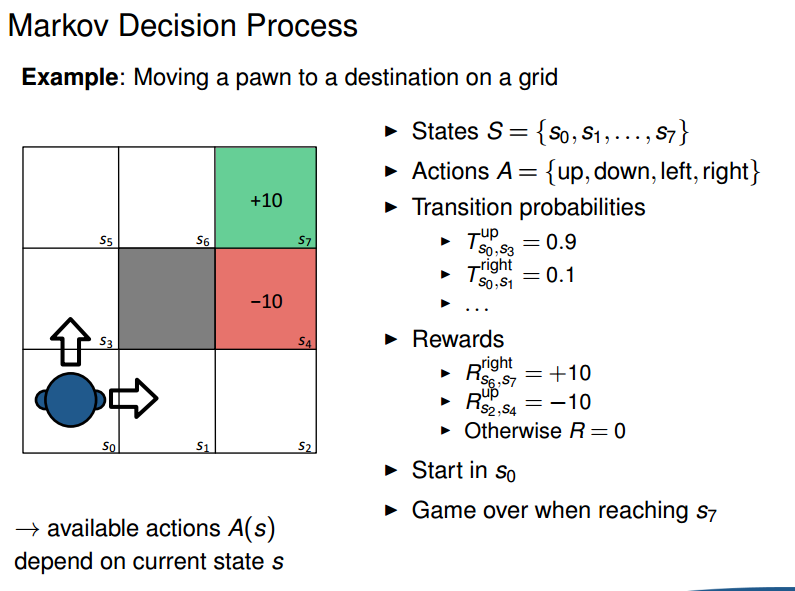
\includegraphics[width=0.7\textwidth]{img/exMdp.png}
        \caption{Caption}
        \label{fig:my_label}
    \end{figure}
\end{frame}

\begin{frame}{Framework de Aprendizado por Reforço (MDP)}
    \begin{figure}
        \centering
        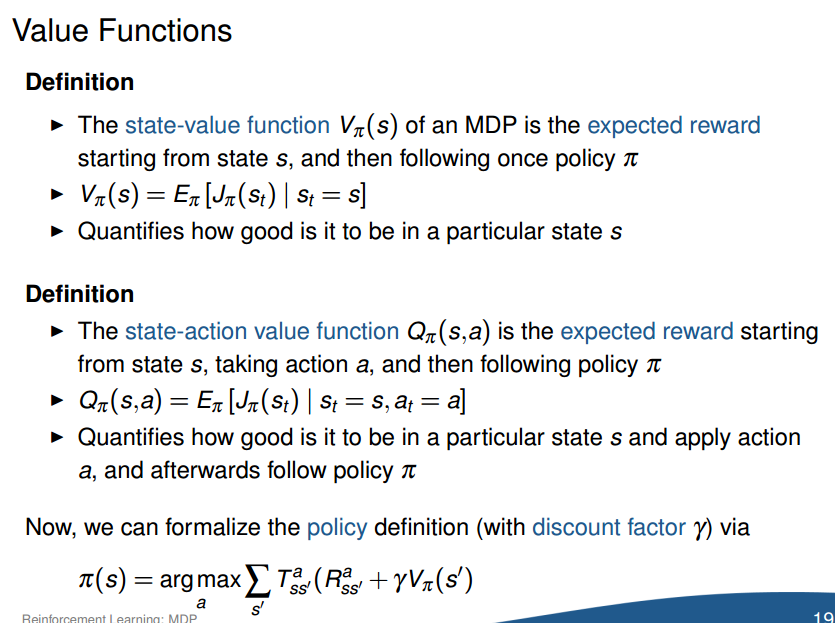
\includegraphics[width=0.7\textwidth]{img/valueFunctions.png}
        \caption{Caption}
        \label{fig:my_label}
    \end{figure}
\end{frame}

\begin{frame}{Framework de Aprendizado por Reforço (MDP)}
    \begin{figure}
        \centering
        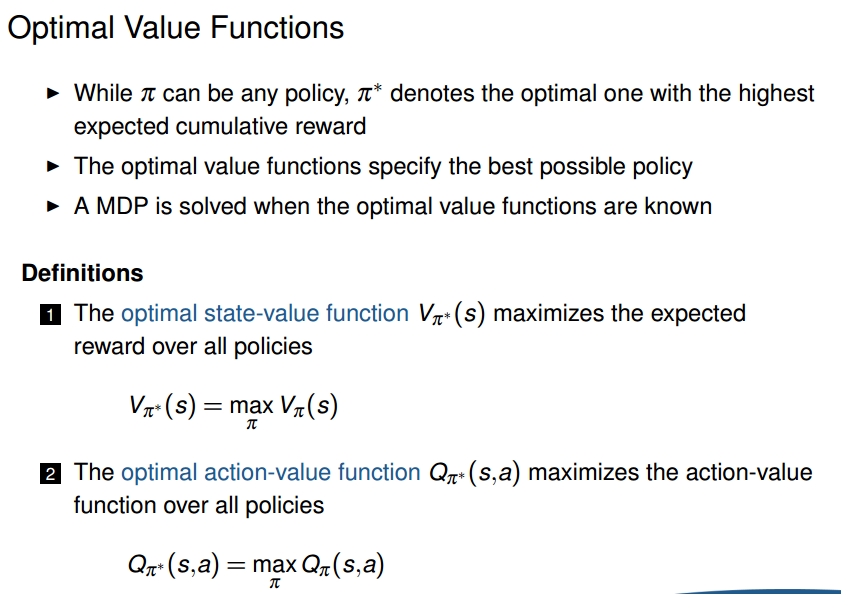
\includegraphics[width=0.7\textwidth]{img/optimal_value_functions.png}
        \caption{Caption}
        \label{fig:my_label}
    \end{figure}
\end{frame}

\begin{frame}{Framework de Aprendizado por Reforço (MDP)}
    \begin{figure}
        \centering
        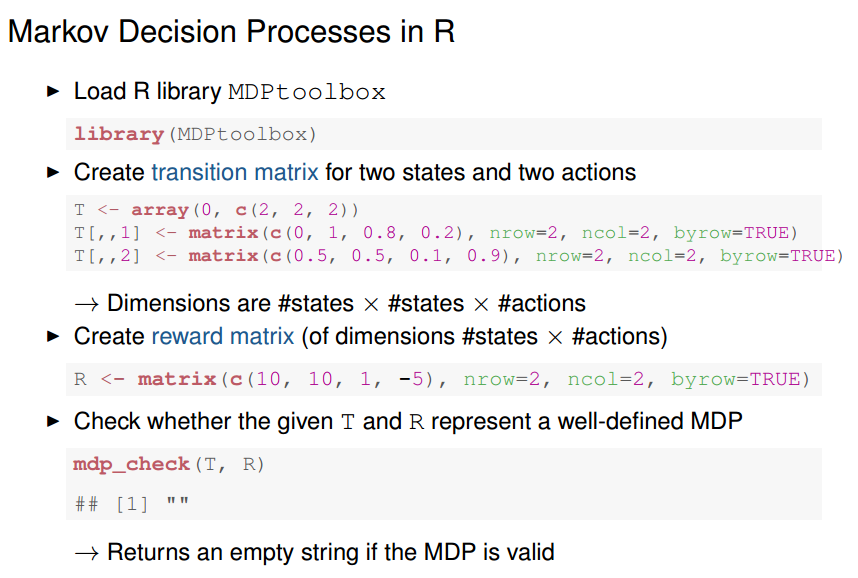
\includegraphics[width=0.7\textwidth]{img/codeMdp.png}
        \caption{Caption}
        \label{fig:my_label}
    \end{figure}
\end{frame}

\begin{frame}{Framework de Aprendizado por Reforço (MDP)}
    \begin{figure}
        \centering
        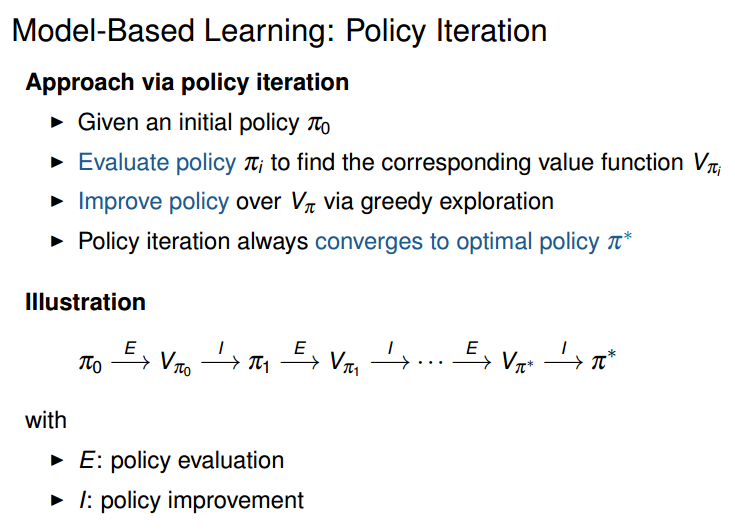
\includegraphics[width=0.7\textwidth]{img/policyIteration.png}
        \caption{Caption}
        \label{fig:my_label}
    \end{figure}
\end{frame}

\begin{frame}{Framework de Aprendizado por Reforço (MDP)}
    \begin{figure}
        \centering
        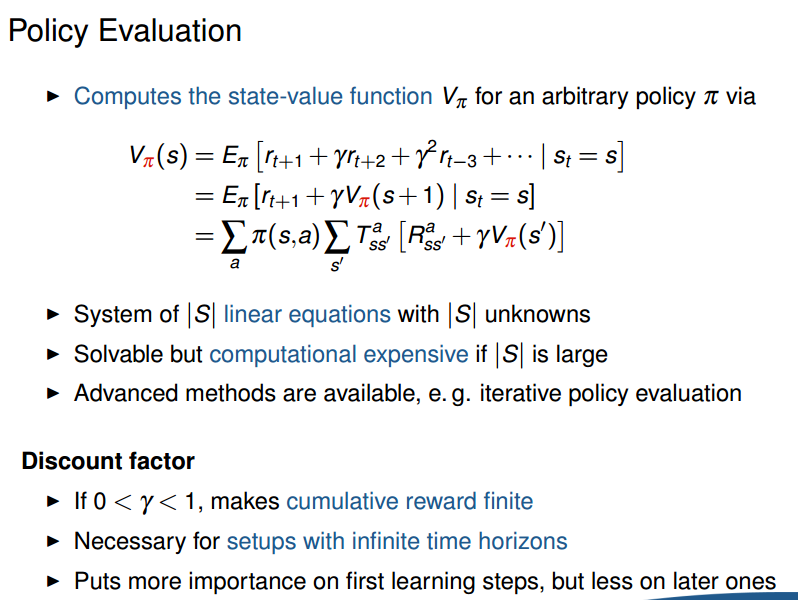
\includegraphics[width=0.7\textwidth]{img/policyEvaluation.png}
        \caption{Caption}
        \label{fig:my_label}
    \end{figure}
\end{frame}

\begin{frame}{Framework de Aprendizado por Reforço (MDP)}
    \begin{figure}
        \centering
        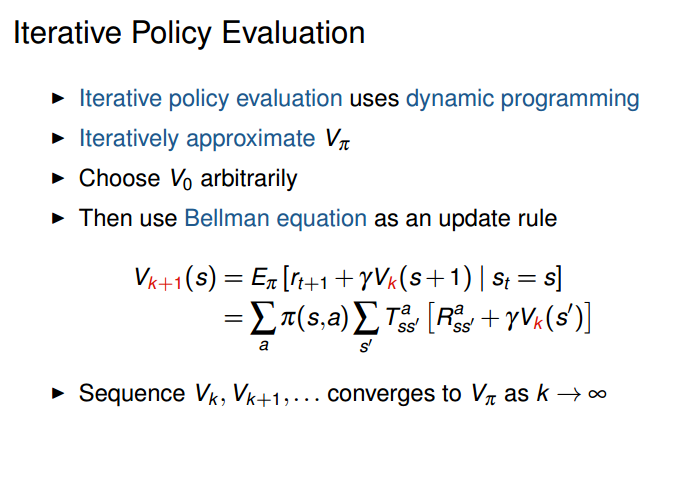
\includegraphics[width=0.7\textwidth]{img/iterativePolicyEvaluation.png}
        \caption{Caption}
        \label{fig:my_label}
    \end{figure}
\end{frame}

\begin{frame}{Framework de Aprendizado por Reforço (MDP)}
    \begin{figure}
        \centering
        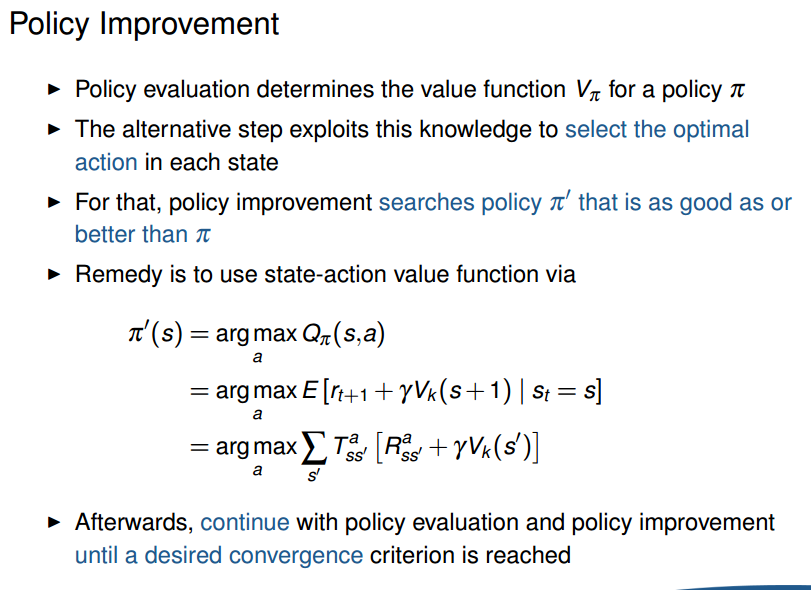
\includegraphics[width=0.7\textwidth]{img/policyImprovement.png}
        \caption{Caption}
        \label{fig:my_label}
    \end{figure}
\end{frame}

\begin{frame}{Framework de Aprendizado por Reforço (MDP)}
    \begin{figure}
        \centering
        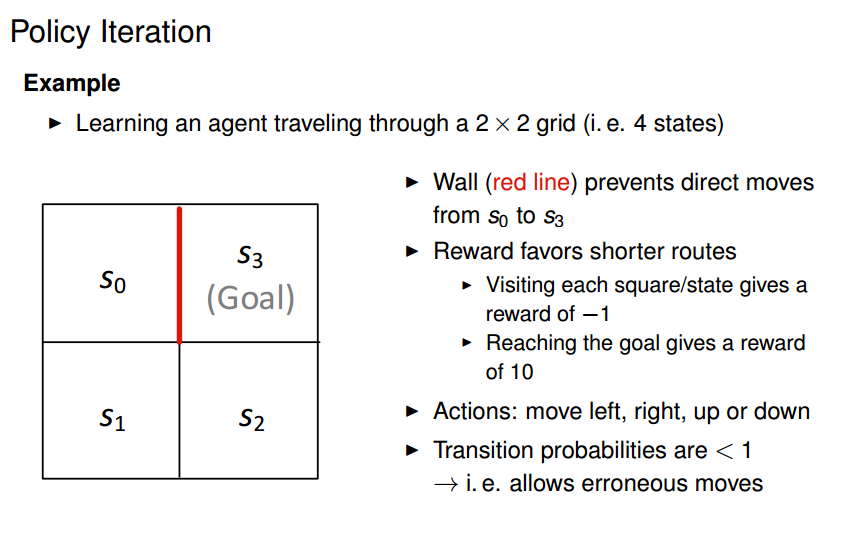
\includegraphics[width=0.7\textwidth]{img/policyIterationExample.png}
        \caption{Caption}
        \label{fig:my_label}
    \end{figure}
\end{frame}

\begin{frame}{Framework de Aprendizado por Reforço (MDP)}
    \begin{itemize}
        %\justifying
        
        \item It is a theorem (Blackwell, 1962) that the optimal infite horizon policy is stationary. \nocite{thesis600} %[p.~20]
        
        %\item TD prediction estimates the state-value function $V_\pi(s)$. For \alert{control}, we must estimate the state-action value function $Q_\pi(s, a)$ instead, so we can do model-free policy improvement and find the optimal policy $π^*$. 
        
    \end{itemize}
\end{frame}

%REVISAR EXPLICAR NA PAG 38 THESIS600
\begin{frame}{Framework de Aprendizado por Reforço (MDP)}
    \textbf{Estados}
    \begin{itemize}
        \item um estado $s_t$ é a representação do ambiente no passo de tempo $t$
        \item pode ser diretamente observado pelo agente ou ser escondido
    \end{itemize}
    \textbf{Ações}
    \begin{itemize}
        \item a cada estado, o agente pode realizar uma ação $a_t$ que afeta o estado subsequente $s_{t+1}$
        \item as ações podem ser qualquer decisão que se deseja aprender
    \end{itemize}
    \textbf{Probabilidades de transição}
    \begin{itemize}
        \item dados um estado s, um possível próximo estado s' e uma ação a
        \item a probabilidade de transição $T_{ss'}^{a}$ de s para s' é definida por $T_{ss'}^{a} = P[s_{t+1} = s' | s_t = s, a_t = a]$
    \end{itemize}
\end{frame}

\begin{frame}{Framework de Aprendizado por Reforço (MDP)}
    \textbf{Recompensa}
    \begin{itemize}
        \item uma recompensa $r_{t+1}$ é um sinal de \alert{retroalimentação} escalar emitido pelo ambiente
        \item indica quão bem o agente está performando para atingir o passo t + 1
        \item a\alert{ recompensa esperada $R_{ss'}^{a}$} quando está se movendo de um estado s para s' via ação a é dada por $R_{ss'}^{a} = E[r_{t+1} | s_t = s, a_t = a, s_{t+1}=s']$
    \end{itemize}
\end{frame}
    
    
    
    